%!TEX root=main.tex

\subsection{Representação do tabuleiro}

\subsubsection{Array Unidimensional (usada no projeto principal)}

Na representação que decidimos usar um tabuleiro de Pentago é um array unidimensional indexado dado por:
\begin{equation*}
3Qx+18Qy+Px+6Py	\qquad\qquad Qx,Qy\in{0,1} \land x,y\in{0,2}.
\end{equation*}
Onde Qx e Qy indicam qual o quadrante e x e y a posição dentro do quadrante. A figura seguinte ilustra melhor como são mapeados os indexes do array no tabuleiro:

\begin{table}[H]
\centering
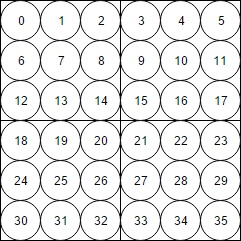
\includegraphics[height=4cm]{images/boardindexes.jpg}
\end{table}

Na prática, no código desenvolvido, não usamos $Qx$ e $Qy$ mas apenas uma única variável para escolher um quadrante quando necessitamos de realizar operações no tabuleiro. A lógica subjacente continua a mesma, apenas mais ofuscada, fazendo a indexação de quadrantes analogamente à leitura de texto (da esquerda para direita e de cima para baixo).

Além do array, na implementação, incluímos também o turno, isto é o próximo a jogar, e o estado da jogada, isto é, colocar peça ou rodar quadrante.

\subsubsection{72 bits - versão ``Pandora''}

Uma das formas de representação do tabuleiro considerada foi como uma estrutura de 72 bits (9 bytes) que podem ser usados, na linguagem de programação usada, com apenas duas variáveis: uma do tipo \verb|long| e outra do tipo \verb|char|. 

Para cada posição do tabuleiro são utilizados 2 bits, sendo que apenas 3 das 4 possíveis configurações de bits seriam usadas. Como o tabuleiro tem 36 posições, ao todo são necessários $2 * 36 = 72$ bits.

Apesar de não ser usada no projeto principal, esta representação foi implementada em \emph{PentagoPandora.cs}~(\ref{PandoraDescricao}).

\subsubsection{55 bits - apenas teorizado}

Removendo simetrias, o número de estados que um jogo de Pentago pode ter é 3.009.081.623.421.558. Isto significa que o número de estados pode ser representado em 52bits, mais alguns extra para representar as simetrias. Se houver um algoritmo que permita inferir os tabuleiros fazendo uso da gama de números de 0 ao valor acima, é possível representar um tabuleiro numa única variável que poderia ser útil para poupar recursos de memória. Tal hipótese levou a algum investimento na consideração das diferentes representações possíveis do tabuleiro.

Uma das forma de representação que conseguimos teorizar necessitaria de apenas 55 bits para representar o tabuleiro, sendo que qualquer estado possível seria identificado por um número único. Ela consiste em considerar todas as possíveis combinações de peças do tabuleiro, sendo que a busca do estado seria feita por ``camadas", inferindo em cada camada informação sobre o tabuleiro que seria usada também nas camadas seguintes. Esta forma teria um número reduzido de estados impossíveis, que representam estados de tabuleiro aparentemente corretos mas que nunca poderiam ser atingidos devido às condições de fim de jogo, sendo por isso bastante compacta. Apesar de poupar memória e ser possível descobrir se 2 estados de tabuleiro são iguais rapidamente, saber qual o tabuleiro que um número representa seria pouco eficiente pelo que a ideia foi descartada do ponto de vista de implementação. Apresentamos contudo uma representação de como se poderia inferir o estado do tabuleiro a partir de um número na gama de 55 bits e qual a fórmula usada no cálculo do número de estados.

\begin{table}[H]
\centering
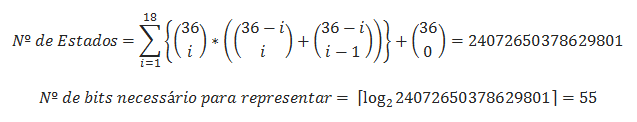
\includegraphics[width=12cm]{images/pentago_rep0.png}

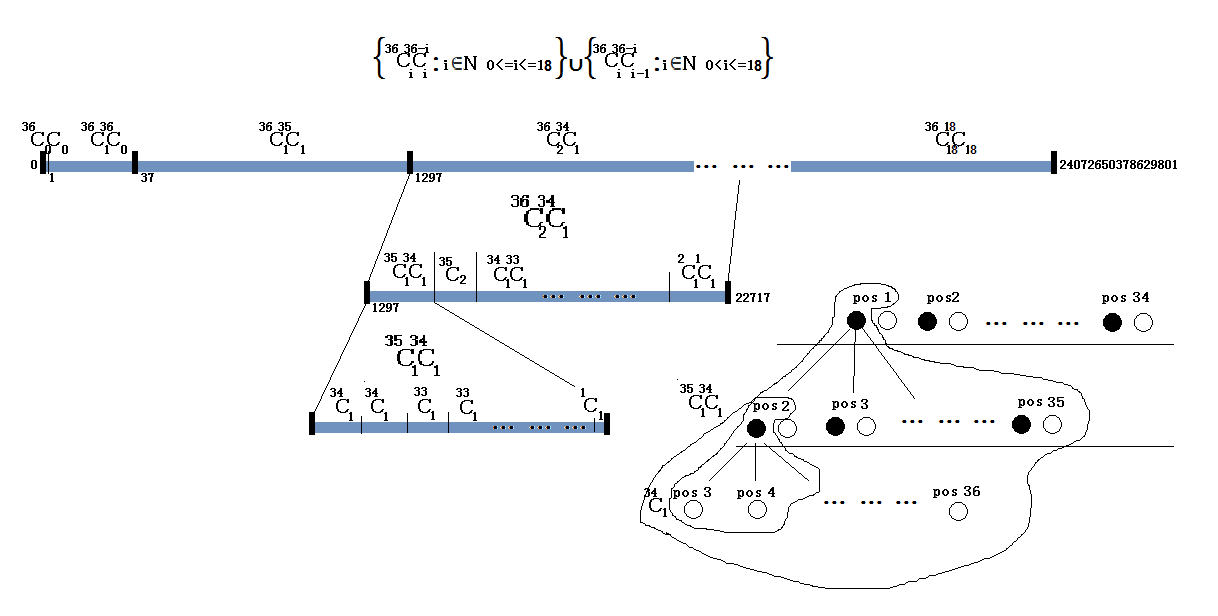
\includegraphics[height=9cm]{images/complex.png}
\end{table}